\chapter{Deep Neural Network Compression}
\label{chap:sota}


\localtableofcontents

\section{Introduction}
\section{Industrial Context}
    \subsection{Smart Home Devices}
    \subsection{Operaitonal Constraint}
% \section{Deep Neural Network Compression}
\section{Deep Learning overview}
\section{Teaching Paradigm}
\section{Architecture Design}
    \subsection{Efficient Architecture}
    \subsection{Neural Architecture Search}
\section{Architecture redfinement}
\subsection{Weight Operations}
\subsection{Pruning}


% \section*{Introduction}
% % region: intro
% The development of neural networks and the enhancement of their performances has
% been accompanied by a significant growth of their size, particularly in the
% number of weights constituting them. In parallel, the evolution of these
% networks has given rise to various applications, particularly embedded ones,
% whose resources are highly constrained in terms of computing power, energy
% consumption or memory footprint. Alongside the increase in the size of these
% networks, compression techniques have been devised, in order to enable the use
% of these algorithms in the said applications. This chapter focuses on these
% techniques and presents state-of-the-art neural network compression methods,
% predominantly based on reducing the number of weights. First, we will explore
% ad-hoc architectures, referred to here as \emph{Efficient Architectures}. These
% networks are lightweight networks that revolve around a core technique to reduce
% their size while preserving performance as much as possible. Following this, we
% will discuss \ac{NAS}, a method that automates the discovery of optimal network
% architectures tailored to specific tasks or constraints, potentially leading to
% more compact and efficient designs. Thereafter, we will examine fast convolution
% techniques, which aim to accelerate the computation of convolutions in neural
% networks, thereby reducing both the runtime and computational resources
% required. Subsequently, we will delve into \ac{KD}, a process by which the
% knowledge of a larger, more complex network (denoted the \emph{teacher}) is
% transferred to a smaller, more efficient network (denoted the \emph{student}),
% enabling the latter to achieve comparable performance with a reduced footprint.
% Afterwards, we will address weight operations techniques, including methods such
% as low-rank factorisation and other linear algebra techniques, which aim to
% reduce the complexity and size of the networks by capitalising on inherent
% redundancies and structures in the weight matrices. Lastly, we will consider
% Neural Network Pruning, a set of techniques that involve the removal of
% redundant or insignificant connections and weights from the network, resulting
% in a sparser and more computationally efficient model.\\

% % TODO: reorganiser le paragraphe précédent qui introduit les sections dont on
% % va parler. Il faut être sûr que ça correspond aux sections qui suivent.

% % endregion: intro

% \section*{Building Blocks for Efficient Architecture Design}

% % region: depthwise separable convolutions

% One of the initial strategies towards achieving efficiency in neural network
% architectures is the use of depthwise separable convolutions. This technique,
% utilised in \cite{howard2017mobilenets} and \cite{DBLP:conf/icml/TanL19},
% separates the standard convolution operation into two distinct steps: a
% depthwise convolution and a pointwise convolution (see
% \cref{fig:sota:depthwise_conv_vs_standard_conv}). By decomposing the operations
% in this manner, the computational complexity is markedly reduced while still
% retaining the ability to capture spatial and channel-wise information. Consider
% an input feature map with $C_\text{in}$ channels of arbitrary width and height
% and $C_\text{out}$ convolution kernels of size $k\times k \times C_\text{in}$. A
% standard convolution algorithm will need $C_\text{in} \times C_\text{out} \times
% k \times k$ \ac{MAC} operations to produce a $1 \times 1 \times C_\text{out}$
% element of the output feature map. In contrast, a depthwise separable
% convolution algorithm will first apply a $k\times k \times 1$ convolution kernel
% to the $C_\text{in}$ channels and then perform $C_\text{out}$ pointwise
% convolutions with $1\times 1 \times C_\text{in}$ kernels to produce the same
% $1\times 1 \times C_\text{out}$ element. This effectively reduces the number of
% parameters to $C_\text{in} \times (C_\text{out} + k \times k)$, essentially
% reducing the number of computations required to produce a $1 \times 1 \times
% C_\text{out}$ element by a factor of\\

% $$\displaystyle\frac{C_\text{out}\times k \times k}{C_\text{out} + k \times k}.$$\\

% \begin{figure}[htbp]
% \centering
% \subfloat[Standard Convolution\label{fig:sota:standard_convolution}]{
%     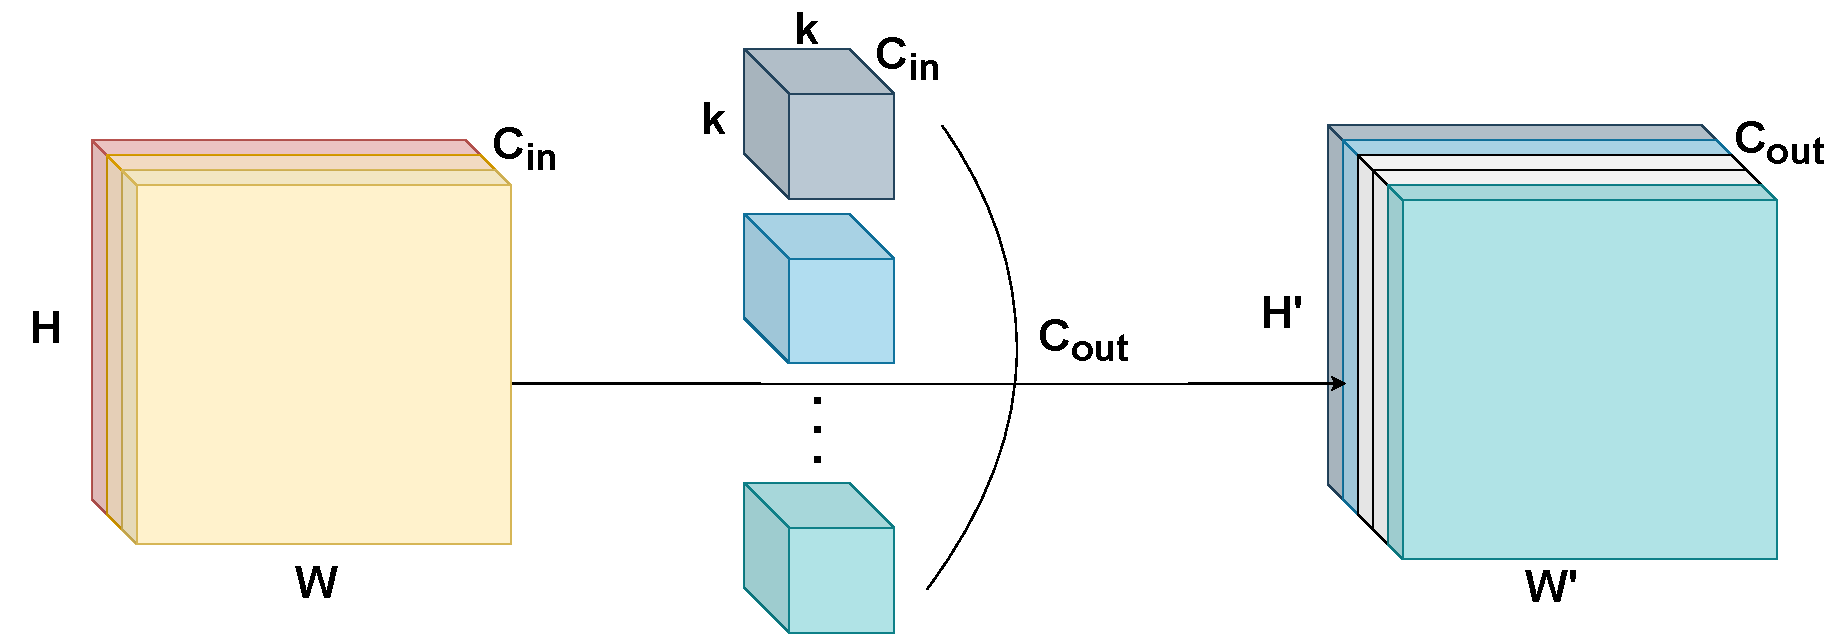
\includegraphics[width=0.70\textwidth]{chapter_sota/assets/standard_conv_scheme.pdf}}\\
%     \vspace{1cm}
% \subfloat[Depthwise Separable
%     Convolution\label{fig:sota:depthwise_convolution}]{
%     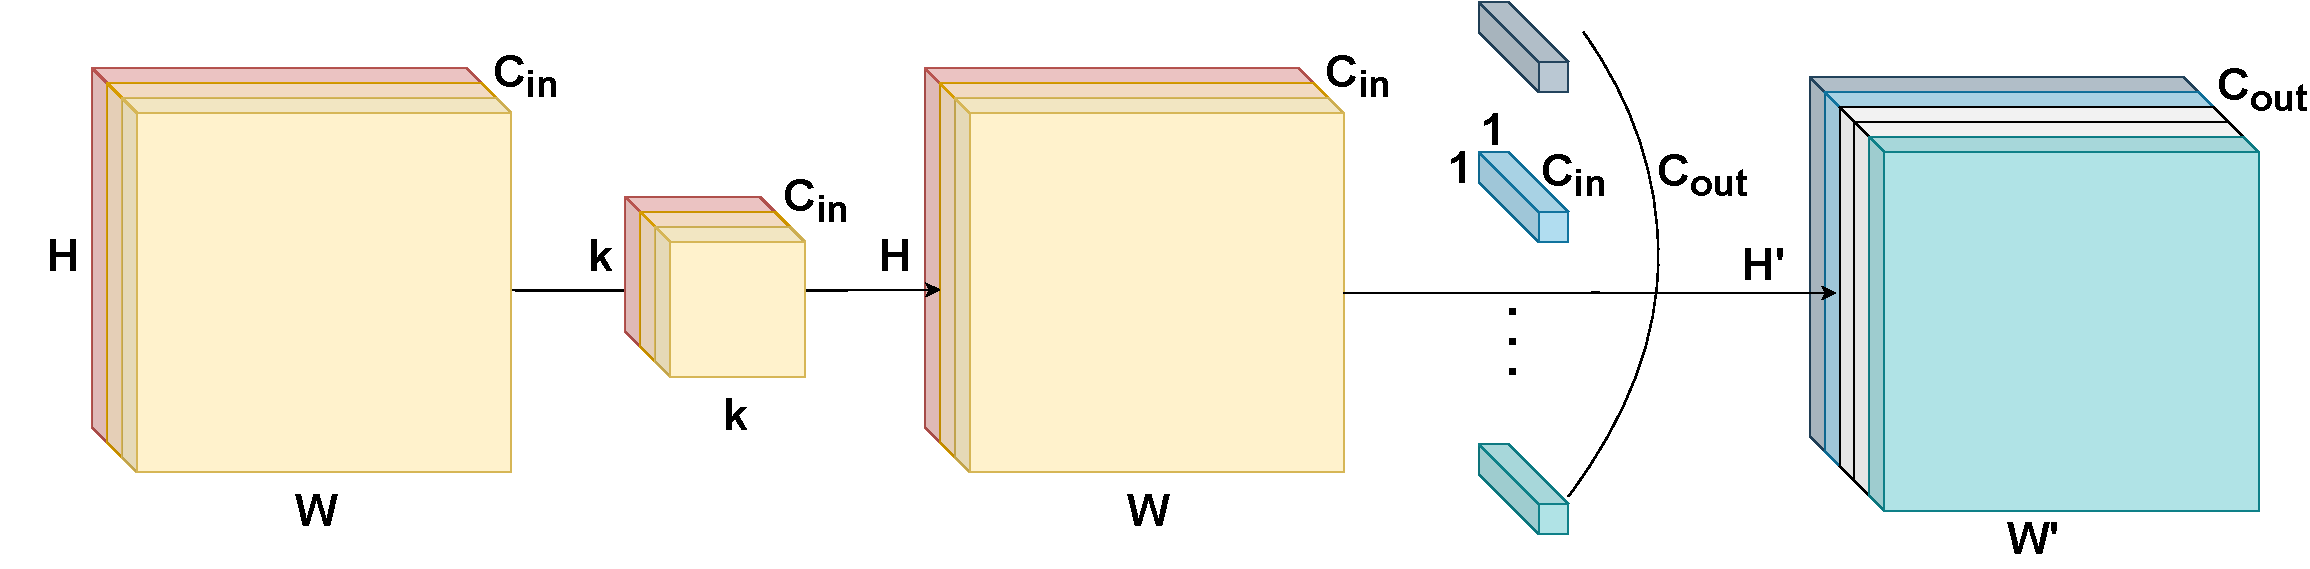
\includegraphics[width=0.70\textwidth]{chapter_sota/assets/depthwise_sep_conv_scheme.pdf}}
%     \caption{Illustration schemes of the standard and depthwise separable
%     convolution. The standard convolution uses $C_\text{out}$ kernels of size
%     $k\times k \times C_\text{int}$. The depthwise separable convolution is
%     split into two steps: \emph{(i)} a convolution with $C_\text{in}$ kernels
%     of size $k \times k$ and \emph{(ii)} a convolution with $C_\text{out}$
%     kernels of size $1\times 1 \times C_\text{int}$.
%     Best viewed in colours.}
% \label{fig:sota:depthwise_conv_vs_standard_conv}
% \end{figure}

% % endregion: depthwise separable convolutions

% % region: fire module
% An alternative approach for designing efficient architectures involves the
% integration of \emph{fire modules}, as proposed in
% \cite{DBLP:journals/corr/IandolaMAHDK16}. These modules aim to minimise
% computational requirements by employing two distinct strategies: \emph{(i)}
% diminishing the number of input channels supplied to the following conventional
% $k\times k$ convolutions and \emph{(ii)} substituting a portion of the
% resource-intensive $k\times k$ convolutions with pointwise convolutions, which
% possess $k^2$ times fewer parameters. The initial strategy is applied within the
% \emph{Squeeze Layer} of the \emph{fire module}, which functions to decrease the
% number of input channels delivered to the \emph{Expand Layer}, subsequently
% reducing the parameter count in the \emph{Expand Layer} kernels. The second
% strategy is implemented in the \emph{Expand Layer}, where some $3\times3$
% convolutions are replaced with $1\times1$ variants. Even though the $1\times1$
% convolutions capture less spatial information, they are significantly less
% computationally demanding.\\

% \begin{figure}[htbp]
%     \centering
%     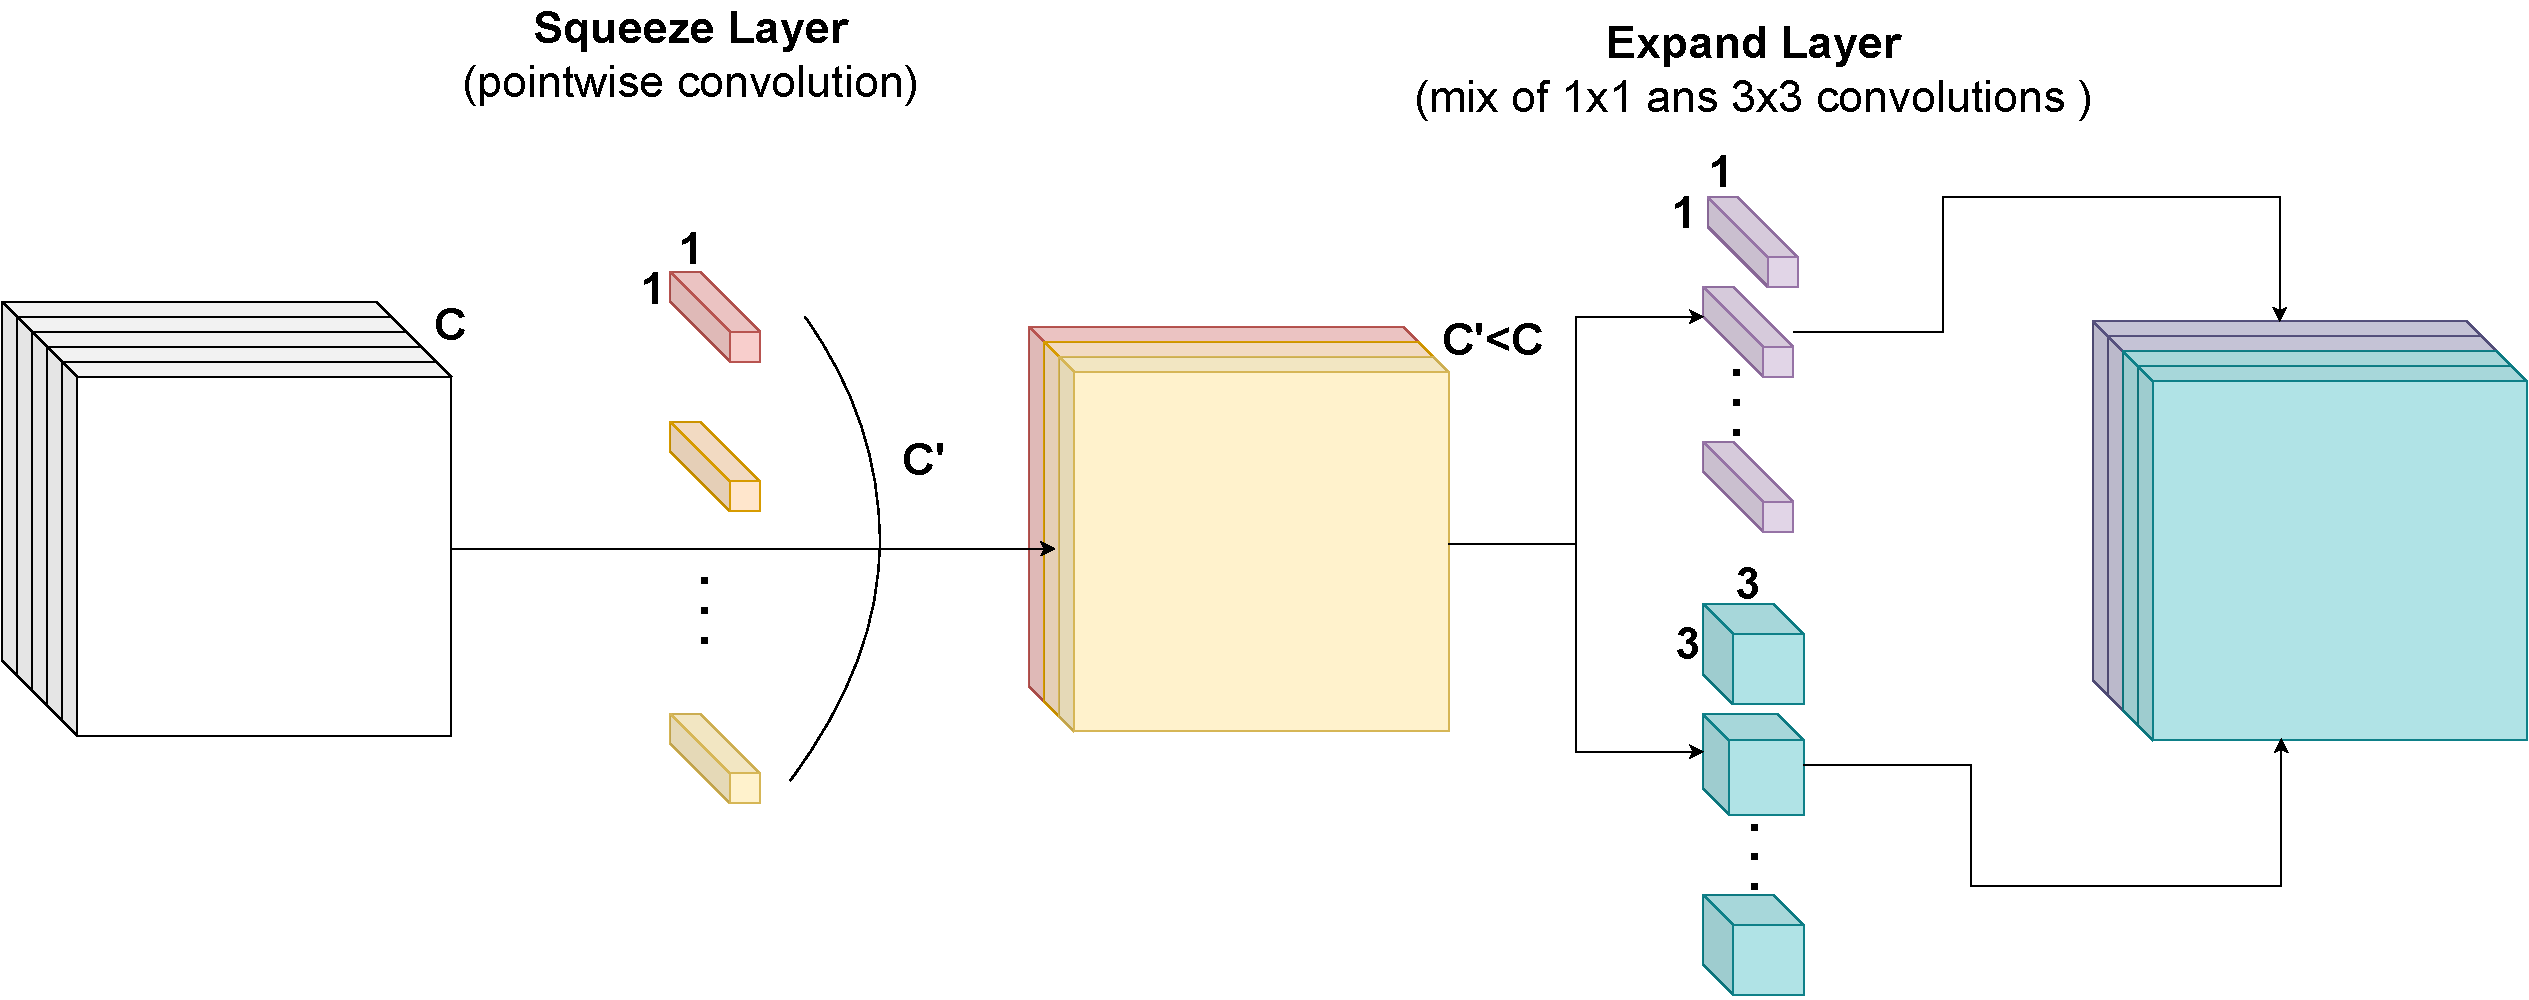
\includegraphics[width=0.70\textwidth]{chapter_sota/assets/fire_module.pdf}
%     \caption{Illustration scheme of the fire module. The fire module is composed
%     is composed of a \emph{squeeze layer} (pointwise convolution designed to
%     reduce the number of channels fed to the following layer) and an
%     \emph{expand layer} (convolution with mixed $1\times1$ and $3\times3$
%     kernels. The $1\times1$ kernels replace some of the $3\times3$ kernels,
%     being less computationally intensive.). Best viewed in colours.}
%     \label{fig:sota:fire_module}
% \end{figure}

% % endregion: fire module

% % region: shufflenet

% Pushing the concept of depthwise separable convolutions further,
% \cite{ZhangShuffleNet} introduces pointwise group convolutions and channel
% shuffle operations to enhance efficiency while maintaining accuracy. Pointwise
% group convolutions were initially introduced in
% \cite{DBLP:conf/nips/KrizhevskySH12}, though their original purpose was not for
% compression. Instead, group convolutions in \cite{DBLP:conf/nips/KrizhevskySH12}
% were used to enable distributed training across multiple \acp{GPU} with limited
% memory. However, ShuffleNet \cite{ZhangShuffleNet} leverages this concept for
% network efficiency by dividing the input channels into groups and performing
% convolutions on each group independently. This approach reduces the number of
% operations and computational cost compared to traditional convolutions. To
% counteract the potential loss of expressive power caused by the separation of
% channels into groups, ShuffleNet incorporates \emph{channel shuffle operations}
% as shown in \cref{fig:sota:shuffle_net}. This technique allows for information
% exchange between groups, effectively maintaining accuracy by ensuring that
% different groups can capture diverse features in the input.\\

% \begin{figure}[htbp]
%     \centering
%     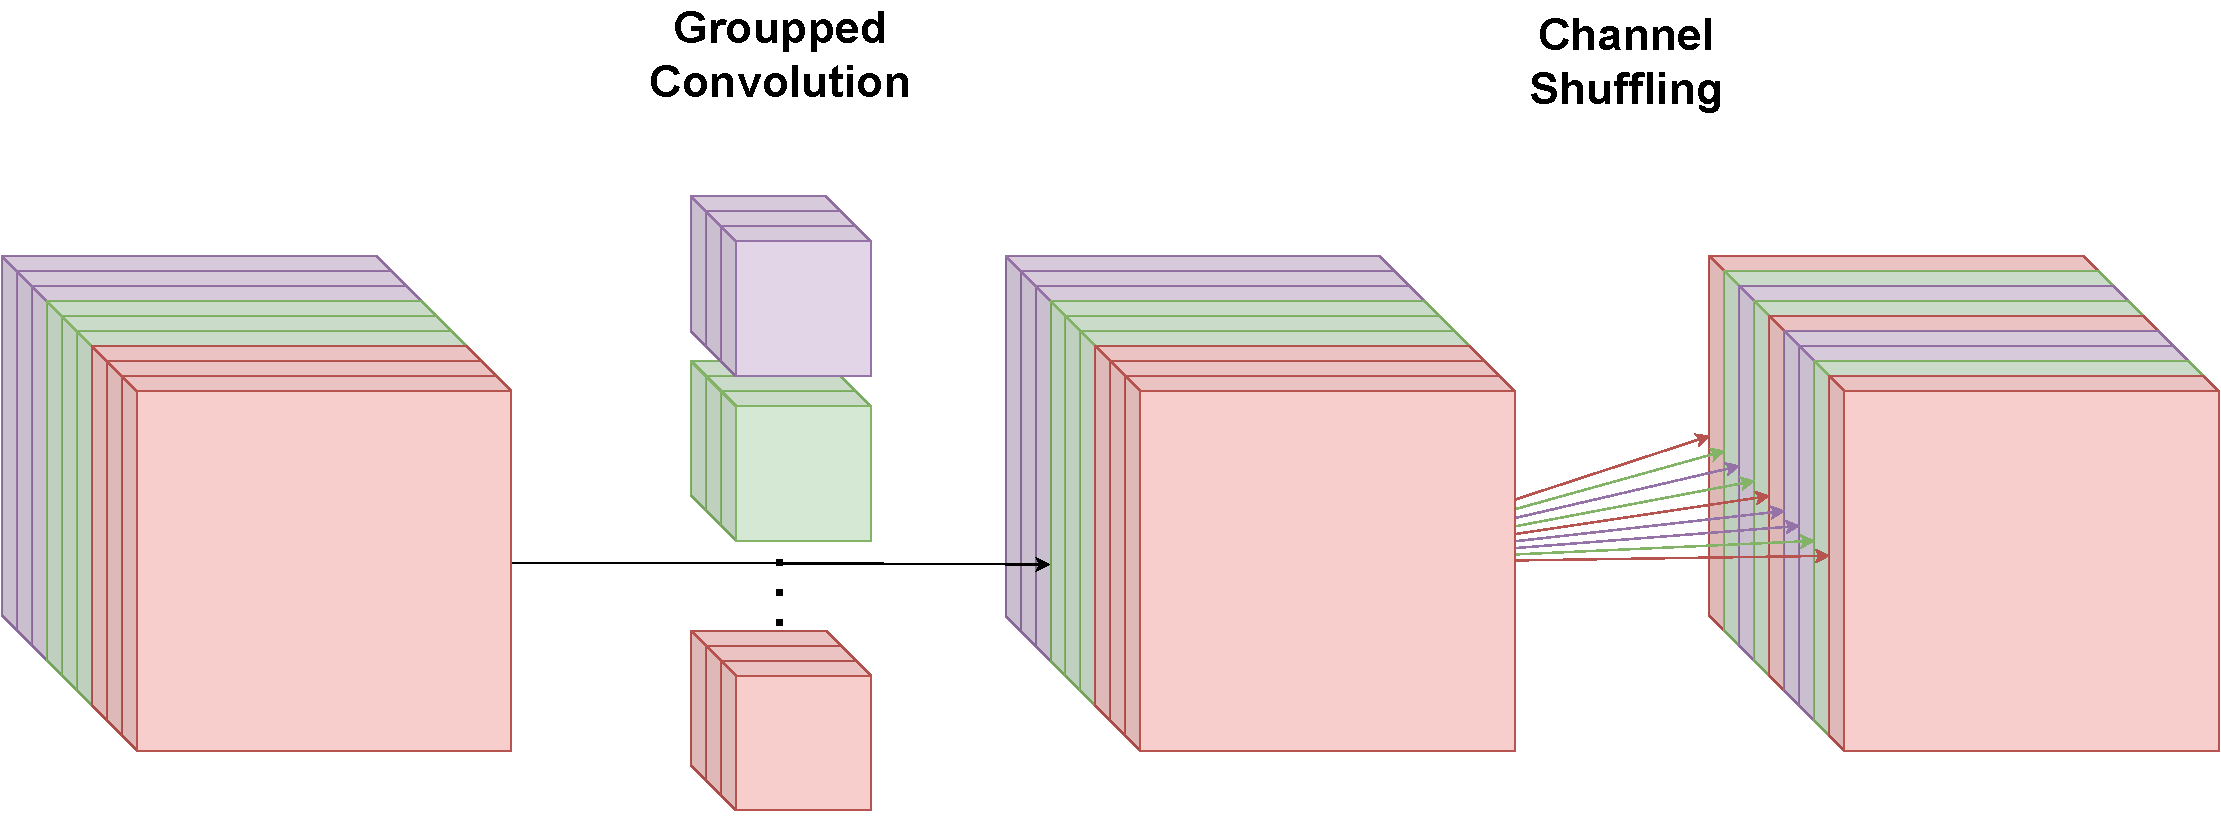
\includegraphics[width=0.70\textwidth]{chapter_sota/assets/group_conv_and_channel_shuffling.pdf}
%     \caption{Illustration scheme of grouped convolution with channel shuffling.
%     Each filter only acts on a subset of the input tensor (here represented by a
%     matching colour). The channels of the yielded tensor are shuffled to ensure
%     the subsequent groups can access information from all the previous groups. Best
%     viewed in colours.}
%     \label{fig:sota:shuffle_net}
% \end{figure}

% Following ShuffleNet, CondenseNet was introduced in \cite{huang2018condensenet},
% incorporating learned group convolutions to further enhance efficiency. Unlike
% the predefined group convolutions in ShuffleNet, CondenseNet learns which
% channels should be grouped together, enabling the network to adapt its structure
% for a specific task. This results in better utilisation of network capacity and
% reduces redundancy. CondenseNet leverages the DenseNet architecture
% \cite{huang2017densely} to further improve performance. Thanks to the densely
% connected architecture, features discarded in any layer can still be recovered
% in subsequent ones.\\

% \begin{figure}[!h]
%     \centering
%     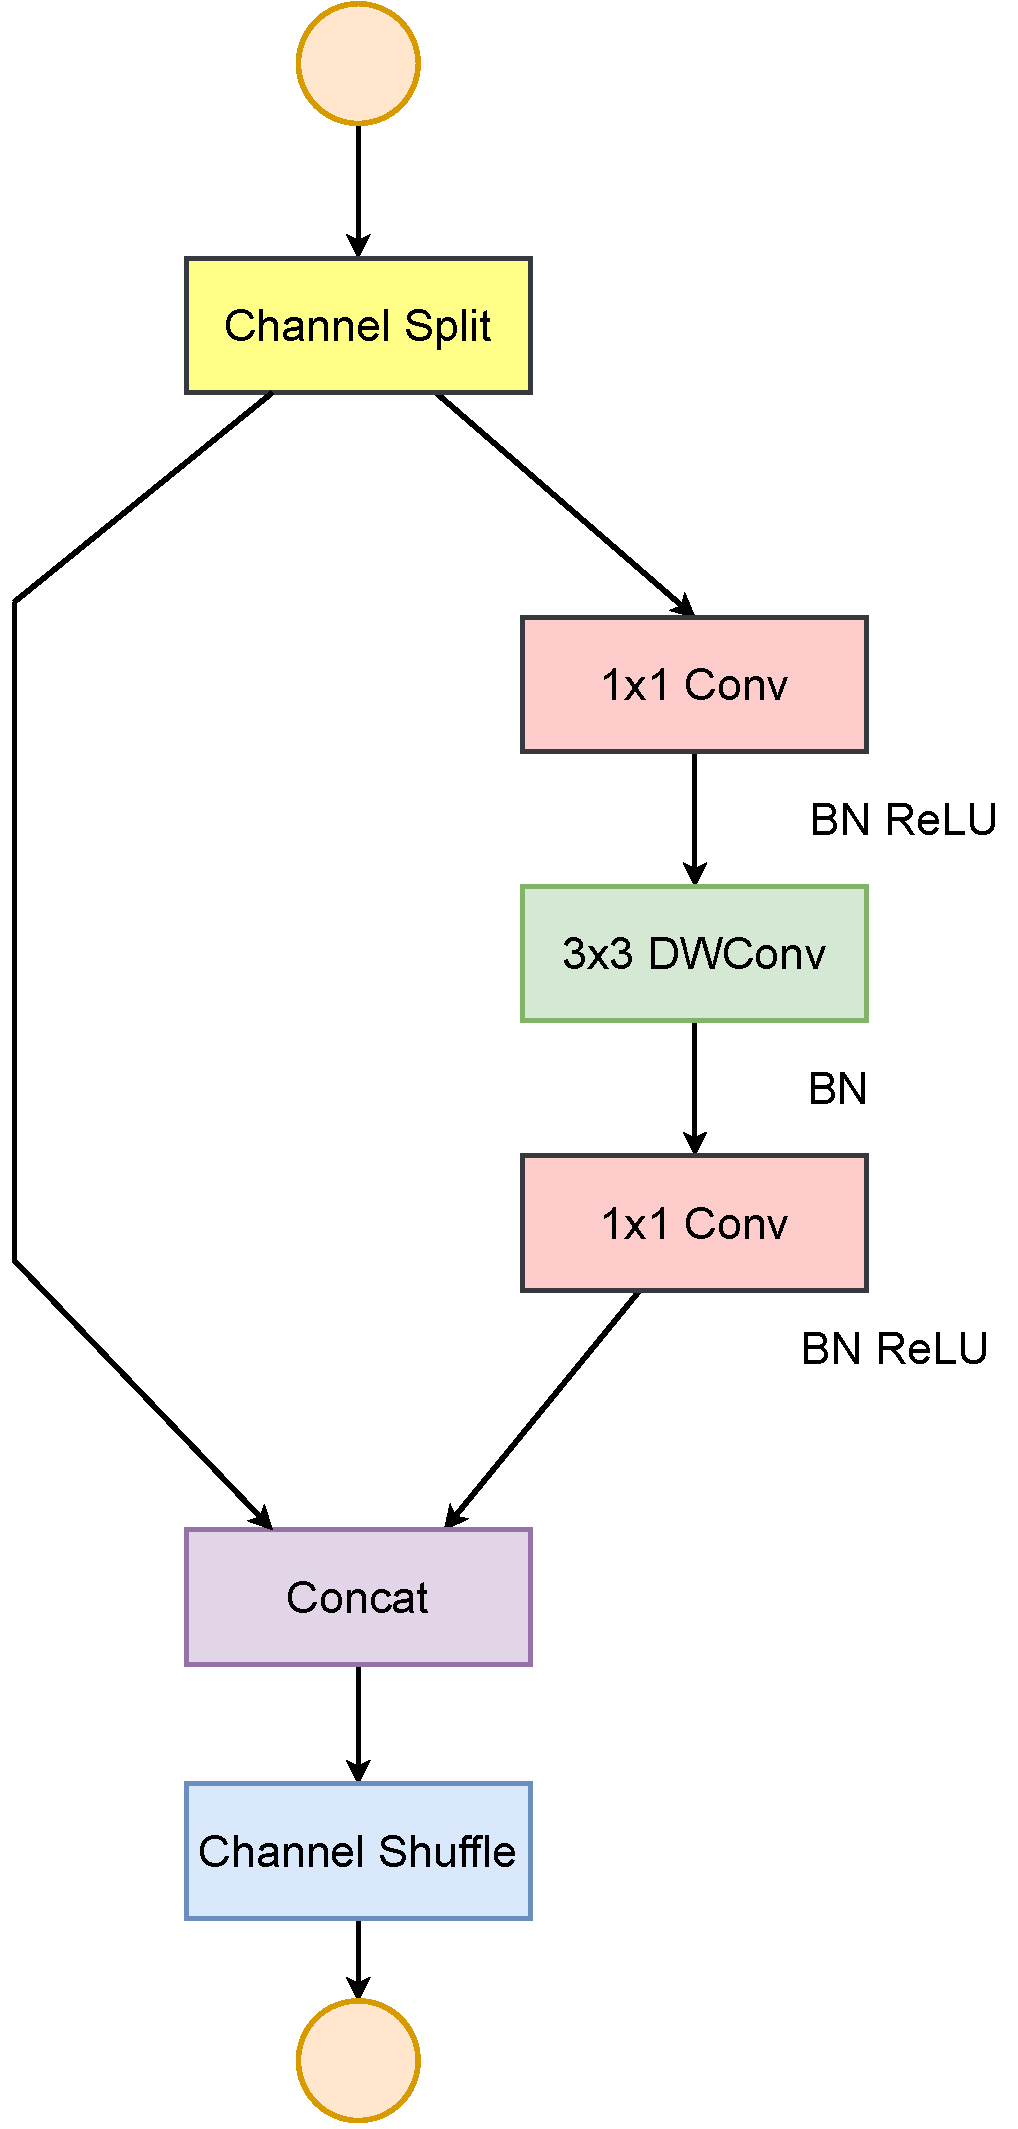
\includegraphics[width=0.3\textwidth]{chapter_sota/assets/channel_split.pdf}
%     \caption{Illustration scheme of the path taken by the feature maps after the
%     channel split block. Adapted from the original scheme found in \cite{MaShuffleNetV2}.}
%     \label{fig:sota:channel_split}
% \end{figure}

% Building on the success of ShuffleNet, ShuffleNetV2 was introduced in
% \cite{MaShuffleNetV2}, focusing on enhancing network efficiency through the
% combination of strided convolution and channel split. Strided convolution helps
% reduce the spatial dimensions of feature maps, thereby reducing the computation
% cost. The Channel Split technique efficiently processes the input feature maps
% while maintaining the expressive power of the architecture. Channel Split works
% by dividing the input feature maps into two equal parts. One part is passed
% through the main branch of the ShuffleNet unit, while the other part is sent
% through the identity branch, which leaves its input unchanged. In the main
% branch, a sequence of pointwise and $3\times 3$ convolutions are performed.
% After both the main branch and the identity branch complete their respective
% operations, the two parts are concatenated along the channel dimension and the
% channels are shuffled. Finally, the output feature maps are passed to the next
% ShuffleNet unit in the network. This process is represented in
% \cref{fig:sota:channel_split}. This approach balances computational efficiency
% with the expressive capacity of the model.\\
% % endregion: shufflenet

% % region: mobilenetv2
% Depthwise Separable Convolutions were employed and improved in
% \cite{howard2017mobilenets}. \citeauthor{DongMobileNetV2} introduced skip
% connections and residual blocks into the MobileNet architecture, initially
% proposed in \cite{DBLP:conf/cvpr/HeZRS16}. They also introduced the concept of
% inverted residuals and linear bottlenecks. In conventional residual blocks, the
% input is first compressed, then expanded, and finally compressed again after
% being added to the original input. With inverted residual bottlenecks, on the
% other hand, this process is reversed: the input is first expanded, then a
% depthwise separable convolution is applied, and finally, it's compressed again.
% In this architecture, the skip connections link the feature maps of smaller
% size, instead of the larger ones. This allows for a more memory-efficient
% architecture. The standard residual blocks and the inverted residual blocks are
% shown in \cref{fig:sota:inverted_vs_residual_blocks}. The linear bottlenecks, on
% the other hand, are convolutions without non-linear activation functions like
% \ac{ReLU}. This takes advantage of the property that high-dimensional feature
% maps can be embedded in a lower-dimensional manifold. To do this, it is
% necessary to use linear transformations without an activation function, which
% could potentially destroy information.\\

% \begin{figure}
%     \centering
%     \subfloat[Standard Residual Block\label{fig:sota:residual_block}]{%
%         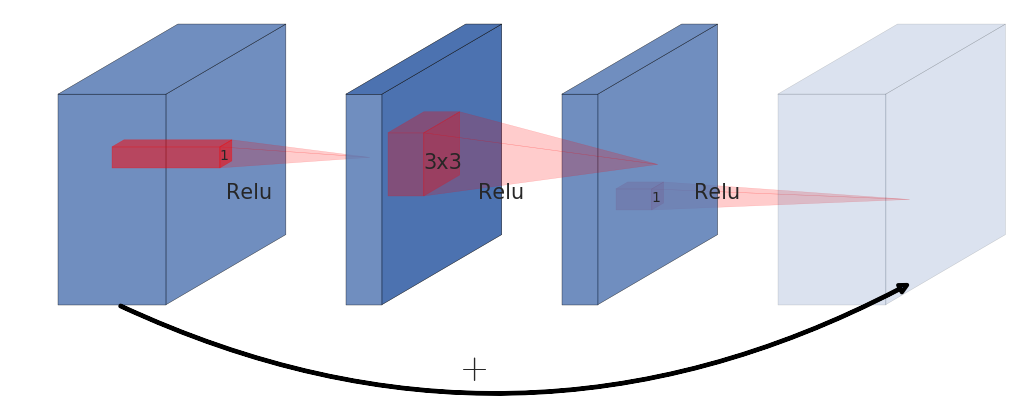
\includegraphics[width=0.49\textwidth]{chapter_sota/assets/mobilenet_v2_residual.png}}
%     \subfloat[Inverted Residual Block\label{fig:sota:inverted_residual_block}]{%
%         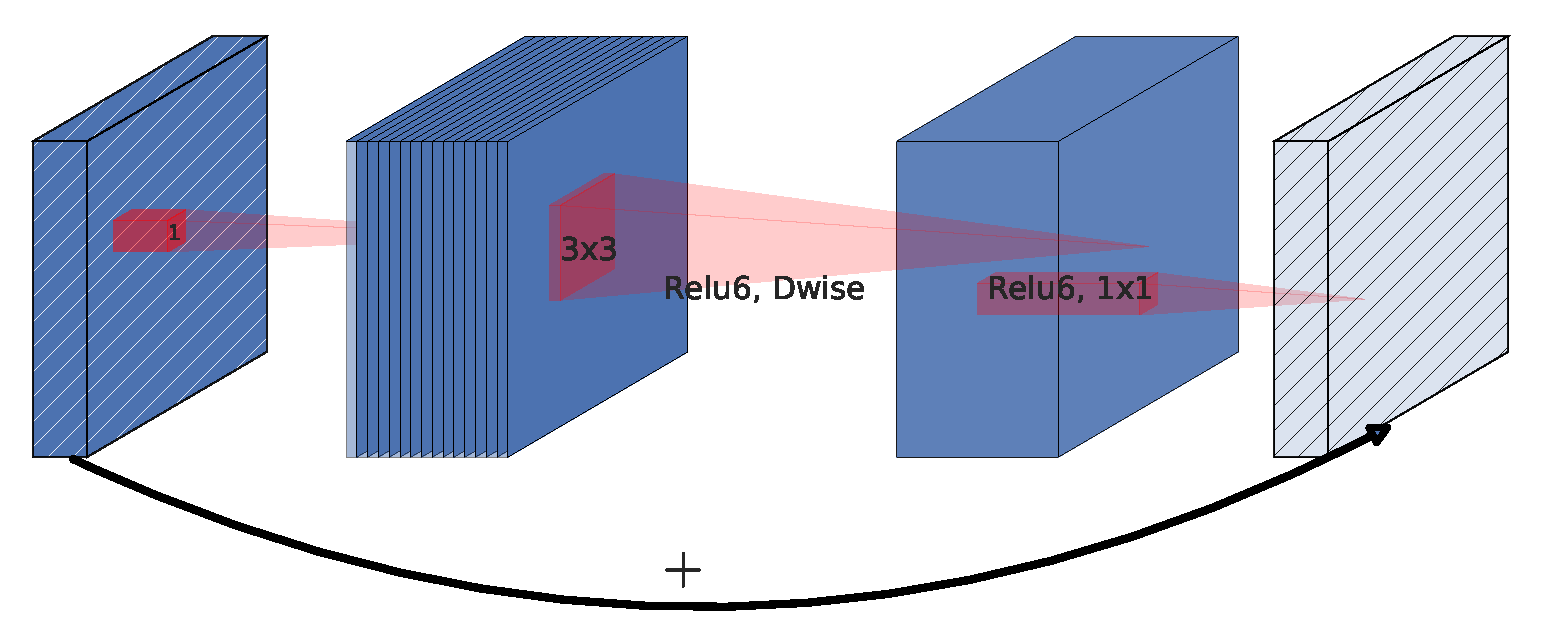
\includegraphics[width=0.49\textwidth]{chapter_sota/assets/mobilenet_v2_inverted_residual.pdf}}
%     \caption{Illustration scheme of the residual block and the inverted residual
%     block. Note that on the inverted residual block, the feature maps with the lower
%     channel count are the ones connected via the skip connection, whereas it is the
%     opposite on the standard residual block. Diagonally hatched layers do not use
%     non-linearities. The grey colour indicates the beginning of the next block. Both
%     illustrations are taken from \cite{DongMobileNetV2}. Best viewed in colours.}
%     \label{fig:sota:inverted_vs_residual_blocks}
% \end{figure}

% % endregion: mobilenetv2

% % region: mobilenetv3
% Advancing from MobileNet and MobileNetV2, its third iteration
% \cite{DBLP:conf/iccv/HowardPALSCWCTC19} incorporated \ac{SE} modules initially
% introduced in \cite{DBLP:conf/cvpr/HuSS18}. These modules adaptively recalibrate
% channel-wise feature responses, amplifying important features and suppressing
% less relevant ones. The \ac{SE} module (represented in
% \cref{fig:sota:se_module}) performs \emph{squeeze} and \emph{excitation}
% operations. The squeeze operation uses global average pooling to create a
% channel descriptor that summarises the spatial information for each channel. The
% excitation operation uses this descriptor to learn non-linear interactions
% between channels through two fully connected layers. The output of this
% mini-network are per-channel modulation weights that recalibrate the original
% feature maps, scaling or "exciting" them by these weights.\\

% % endregion: mobilenetv3

% % region: transition paragraph
% The architectures we have just reviewed revolve around specific key techniques
% such as depthwise separable convolutions, fire modules, channel shuffling, and
% \ac{SE} modules, among others. These architectures, while highly efficient, are
% manually crafted and require a significant degree of human expertise, intuition,
% and time to develop, optimise, and fine-tune. The manual design of these
% architectures often relies on a deep understanding of the tasks at hand, the
% data they will process, and the constraints of the environment in which they
% will operate. However, the process of designing these efficient architectures
% can be automated, which is the subject of the next section.\\


% \begin{figure}[htbp]
%     \centering
%     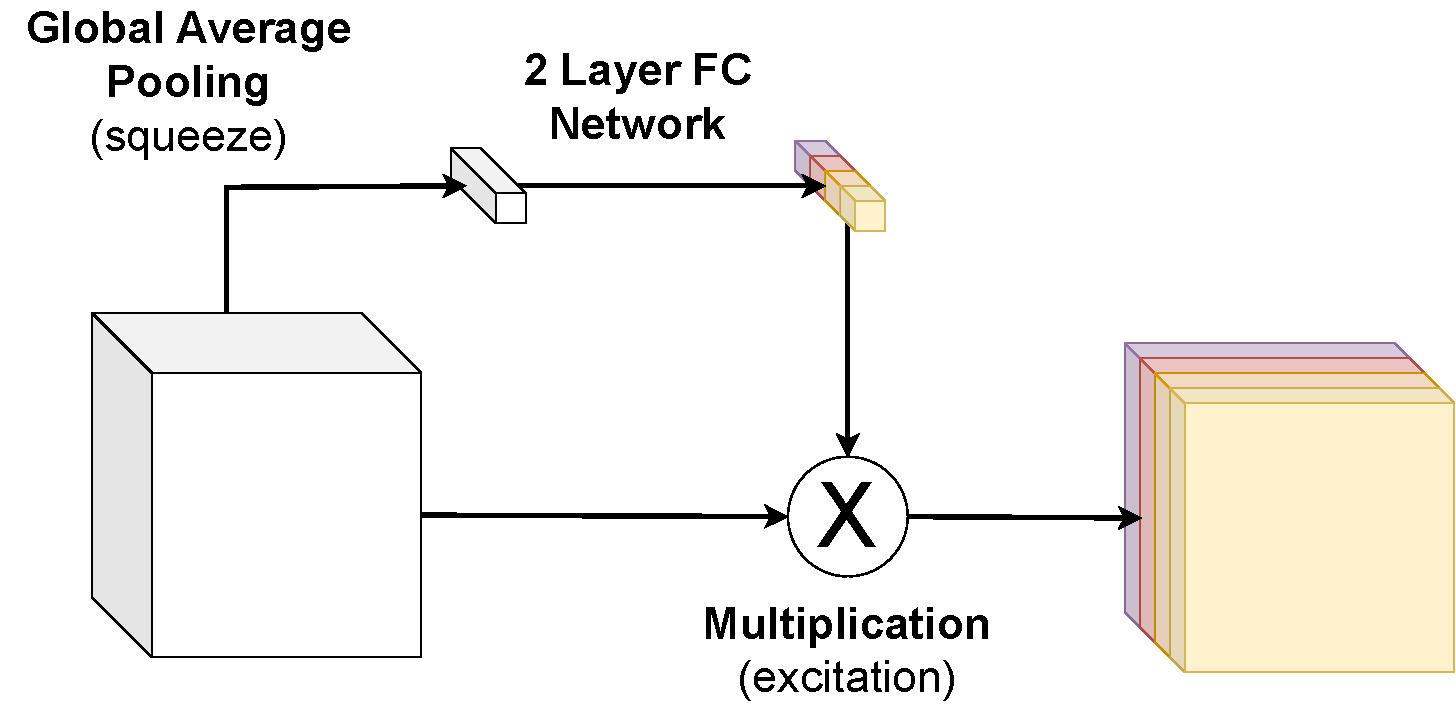
\includegraphics[width=0.70\textwidth]{chapter_sota/assets/SE_module.pdf}
%     \caption{Illustration scheme of the \acf{SE} module. The original feature
%     map is \emph{squeezed} into a channel descriptor through global average
%     pooling. This descriptor is then used to learn the interdependencies between
%     the channels through two fully connected layers. The output is then
%     multiplied layerwise with the original feature map (\emph{excitation}). Best
%     viewed in colours.}
%     \label{fig:sota:se_module}
% \end{figure}

% % endregion: transition paragraph

% \section*{Automatic Architecture Design Through Neural Architecture Search}
% \label{sec:sota:nas} 

% \acf{NAS} is a method that automates the discovery of neural network
% architectures, potentially leading to more compact, efficient designs and
% reducing the need for manual intervention. Although \ac{NAS} might not
% explicitly aim at producing lightweight architectures, it can still yield
% designs that strike a good balance between performance and computational cost
% \cite{DBLP:conf/cvpr/TanCPVSHL19,DBLP:conf/icml/TanL19}. By using automated
% methods to search for optimal architectures, it is possible to further enhance
% the efficiency of neural networks, opening up new possibilities for their
% deployment in resource-constrained environments. \ac{NAS} has emerged as an
% essential paradigm, aiming to automate the traditionally manual and
% labour-intensive process of designing efficient neural networks
% \cite{DBLP:journals/corr/MiikkulainenLMR17}. Early network architectures were
% indeed entirely handcrafted, requiring significant human effort and expertise.
% However, these manual methods are being replaced by \ac{NAS} techniques, which
% seek to automatically determine the optimal network structure given a training
% set \cite{DBLP:journals/corr/abs-2301-08727,elsken2019neural}.\\

% The performance and efficiency of \ac{NAS} are fundamentally determined by two
% key aspects: the \emph{search space} and the \emph{search strategy}. The search
% space, as the term suggests, defines the set of all possible architectures that
% can be discovered by the \ac{NAS} algorithm. It could be as broad as all
% possible configurations of a certain type of network, such as \acp{CNN}, or as
% narrow as different arrangements of a specific set of layers
% \cite{DBLP:conf/cvpr/LiuCSAHY019}. The search strategy, on the other hand,
% determines how the \ac{NAS} algorithm navigates through this search space in
% order to optimise its given objective. This could involve gradient-based
% strategies \cite{DBLP:conf/iclr/LiuSY19,DBLP:conf/iclr/XuX0CQ0X20}, or
% stochastic methods, such as evolutionary algorithms and reinforcement learning
% strategies \cite{DBLP:conf/iclr/ZophL17,DBLP:conf/icml/RealMSSSTLK17}. The
% choice of search space and search strategy significantly influences the ability
% of \ac{NAS} to discover effective and efficient architectures, and is thus a
% critical aspect of NAS research. In the following paragraphs, we will delve
% deeper into some of these strategies and their impact on the field of
% \ac{NAS}.\\



% The search space is a critical aspect of \ac{NAS} as it bounds the possibilities
% of architectures and significantly influences the outcome of the search. The
% search space could be as broad as all possible configurations of a certain
% network type or as specific as various arrangements of a predefined set of
% layers or blocks. For instance, \cite{DBLP:conf/iclr/ZophL17} define their
% search space as a set of repeatable sub-structures composed of basic layers
% (convolution layers, fully connected layers, \ac{batch norm} layers, etc...)
% often called \emph{cells} that are stacked to form the final architecture, while
% \cite{DBLP:conf/iclr/XieZLL19} design their search space based on the
% connectivity patterns between network blocks. \cite{DBLP:conf/iclr/LiuSY19}
% propose a continuous search space where the architecture is parameterized as a
% differentiable function, allowing for efficient search using gradient-based
% methods. Hierarchical search spaces, on the other hand, offer a strategic
% approach to navigate the complexity of the architecture search in \ac{NAS}
% \cite{DBLP:conf/cvpr/LiuCSAHY019,DBLP:conf/cvpr/TanCPVSHL19}. In such a setup,
% the architecture is divided into several levels of hierarchy, with each level
% searched independently. This structure enables a more systematic and organized
% exploration of the search space, allowing the algorithm to uncover useful
% patterns and configurations at different levels of the network. The EfficientNet
% models are exemplary of innovative architecture search strategies
% \cite{DBLP:conf/icml/TanL19}. This series utilizes both \ac{NAS} and
% \emph{compound scaling}. A baseline, EfficientNet-B0, was developed through
% multi-objective \ac{NAS}, optimizing both accuracy and \acp{FLOP}. Subsequently, a
% compound scaling method was applied to this baseline, uniformly scaling depth,
% width, and resolution via a \emph{compound coefficient} $\phi$. This approach
% yielded a series of progressively larger EfficientNet models, whose performances
% are shown in \ref{fig:sota:efficientnet_perfs}.\\\


% \begin{figure}[htbp]
%     \centering
%     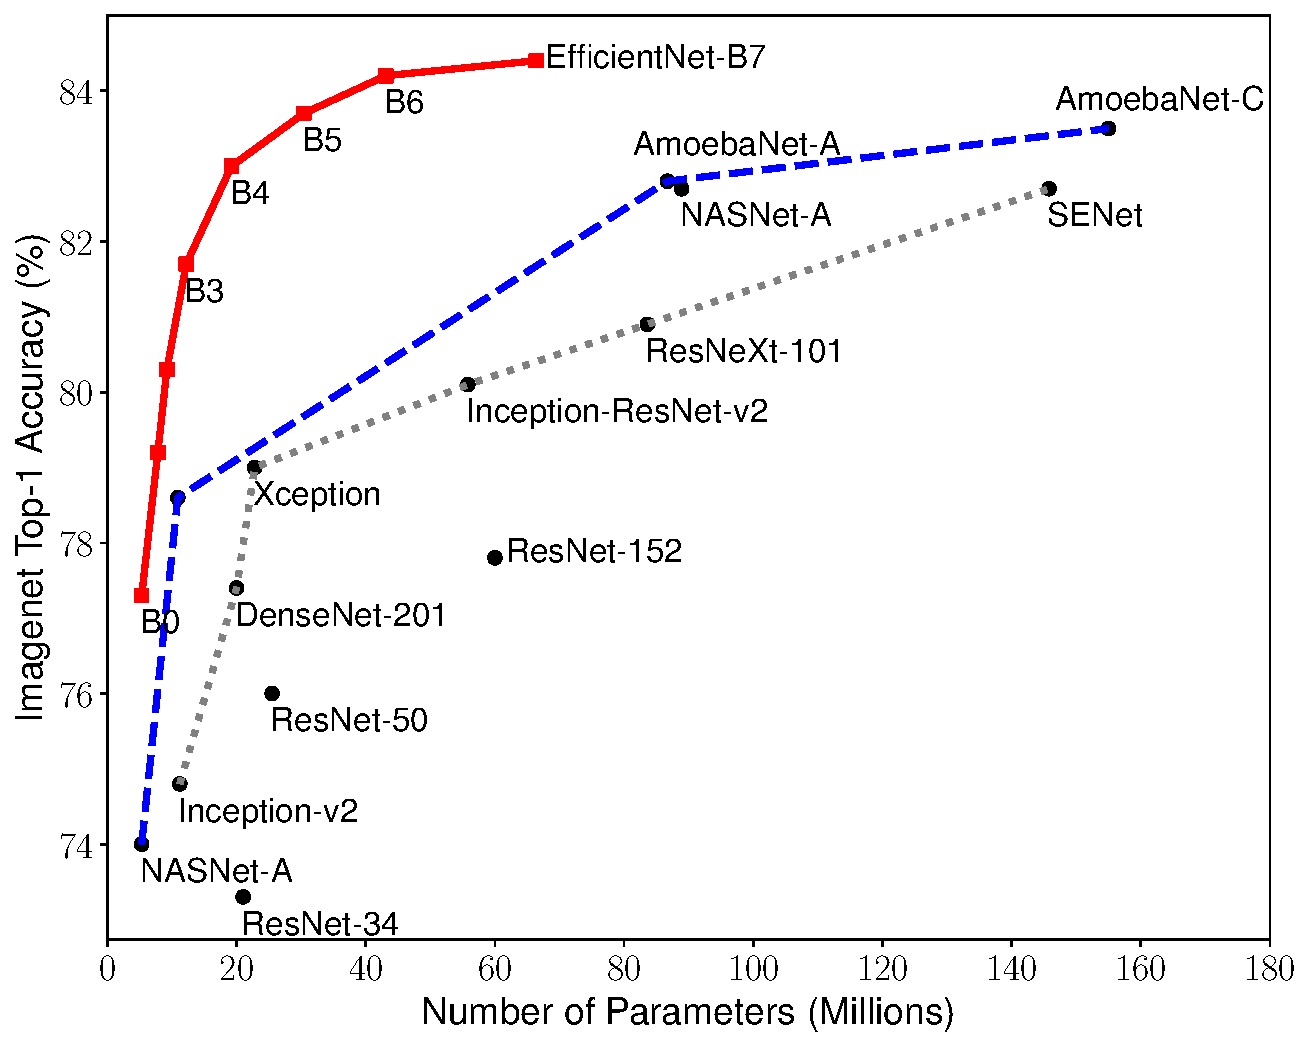
\includegraphics[width=0.70\textwidth]{chapter_sota/assets/efficientnet_perfs_overview.pdf}   
%     \caption{ImageNet top-1 accuracy vs model size (in millions of parameters).
%     The EfficientNet family of models significantly outperforms other models of
%     similar size, obtained either by \ac{NAS} or manual design. This graph is
%     taken from \cite{DBLP:conf/icml/TanL19}.
%     }
%     \label{fig:sota:efficientnet_perfs}
% \end{figure}


% The search strategy is another major component of \ac{NAS}, dictating how the
% algorithm explores the search space to find the optimal architecture. A wide
% range of search strategies have been proposed. Evolutionary algorithms
% \cite{DBLP:conf/icml/RealMSSSTLK17} use principles of natural evolution such as
% mutation, crossover, and selection to explore the search space. Despite their
% potential to find high-quality solutions, these methods often require
% substantial computational resources due to the large number of evaluations
% needed. Reinforcement Learning-based methods \cite{DBLP:conf/iclr/ZophL17}
% employ a policy network to generate architectures and a reward signal, typically
% validation accuracy, to guide the search. While reinforcement learning methods
% can effectively navigate large search spaces, their success heavily depends on
% the quality of the reward signal. Gradient-based methods like
% \cite{DBLP:conf/iclr/LiuSY19,DBLP:conf/iclr/XuX0CQ0X20} make the search space
% continuous and use gradient descent for optimization, which enables efficient
% exploration of the search space but requires careful regularization to prevent
% overfitting. \cite{DBLP:conf/nips/BergstraBBK11} uses Bayesian optimization to
% build a probabilistic model of the objective function and uses it to select
% promising architectures, balancing exploitation and exploration. This method can
% be sample-efficient but might struggle with high-dimensional spaces. These
% diverse strategies offer multiple paths to navigate the complex landscape of
% architecture search, each with its unique trade-offs between efficiency,
% effectiveness, and computational demands.\\

% \section*{Improved Lightweight Model Training with Knowledge Distillation}

% \acf{KD} is a method that aims to transfer the knowledge of a large, complex and
% accurate network referred to as the \emph{teacher} to a smaller, more efficient
% one called the \emph{student}. The student is trained with a combination of the
% main task loss as well as a supplementary supervision signal which is derived
% from the feature maps of the teacher network at various depths.\\

% Methods in this paradigm are mostly based on the seminal work of
% \citeauthor{DBLP:journals/corr/HintonVD15} \cite{DBLP:journals/corr/HintonVD15}.
% The latter seeks to train simple networks with \acl{KD} yielding better
% performances compared to those trained from scratch. \ac{KD} relies on teacher
% and student networks, where the logits of the former are used as an additional
% supervision signal for the latter. When trained separately, the student network
% can only rely on classification labels in order to learn its own data
% representation while \ac{KD} relies on the logits of the teacher network which
% provide more insight about the hidden representations.\\

% Inspired by \ac{KD}, \cite{DBLP:journals/corr/RomeroBKCGB14} introduced FitNet,
% a two-stage training algorithm, where an intermediate layer of the teacher is
% chosen as a \emph{hint}\footnote{\emph{Hint} is the terminology used by
% \citeauthor{DBLP:journals/corr/RomeroBKCGB14}
% \cite{DBLP:journals/corr/RomeroBKCGB14} to denote a feature map used as a target
% for the student network.} for an intermediate layer of the student. First, the
% student is trained up to its selected layer to mimic the hint feature map. Then,
% the whole student network is trained with standard \ac{KD} against the whole
% teacher. In the first step, a regressor is needed in order to adapt the
% dimensions of the feature map, which may differ from the teacher to the student
% networks, as illustrated in \cref{fig:sota:kd_frameworks}.
% \citeauthor{DBLP:conf/cvpr/YimJBK17} argue that the direct feature map matching
% utilised by FitNets is overly restrictive. Drawing inspiration from the
% techniques used in \cite{DBLP:journals/corr/GatysEB15a} for style transfer, they
% propose an alternative method. In the context of style transfer, the Gram matrix
% of the feature maps is employed to encapsulate the texture information of an
% image. Adapting this approach, the method presented in
% \cite{DBLP:conf/cvpr/YimJBK17} calculates the Gram matrix across multiple layers
% feature maps. This computed Gram matrix, dubbed the Flow of Solution Procedure
% (FSP) matrix, then serves as a \emph{hint} for the student network, guiding its
% training process.\\

% \begin{figure}[htbp]
%     \centering
%     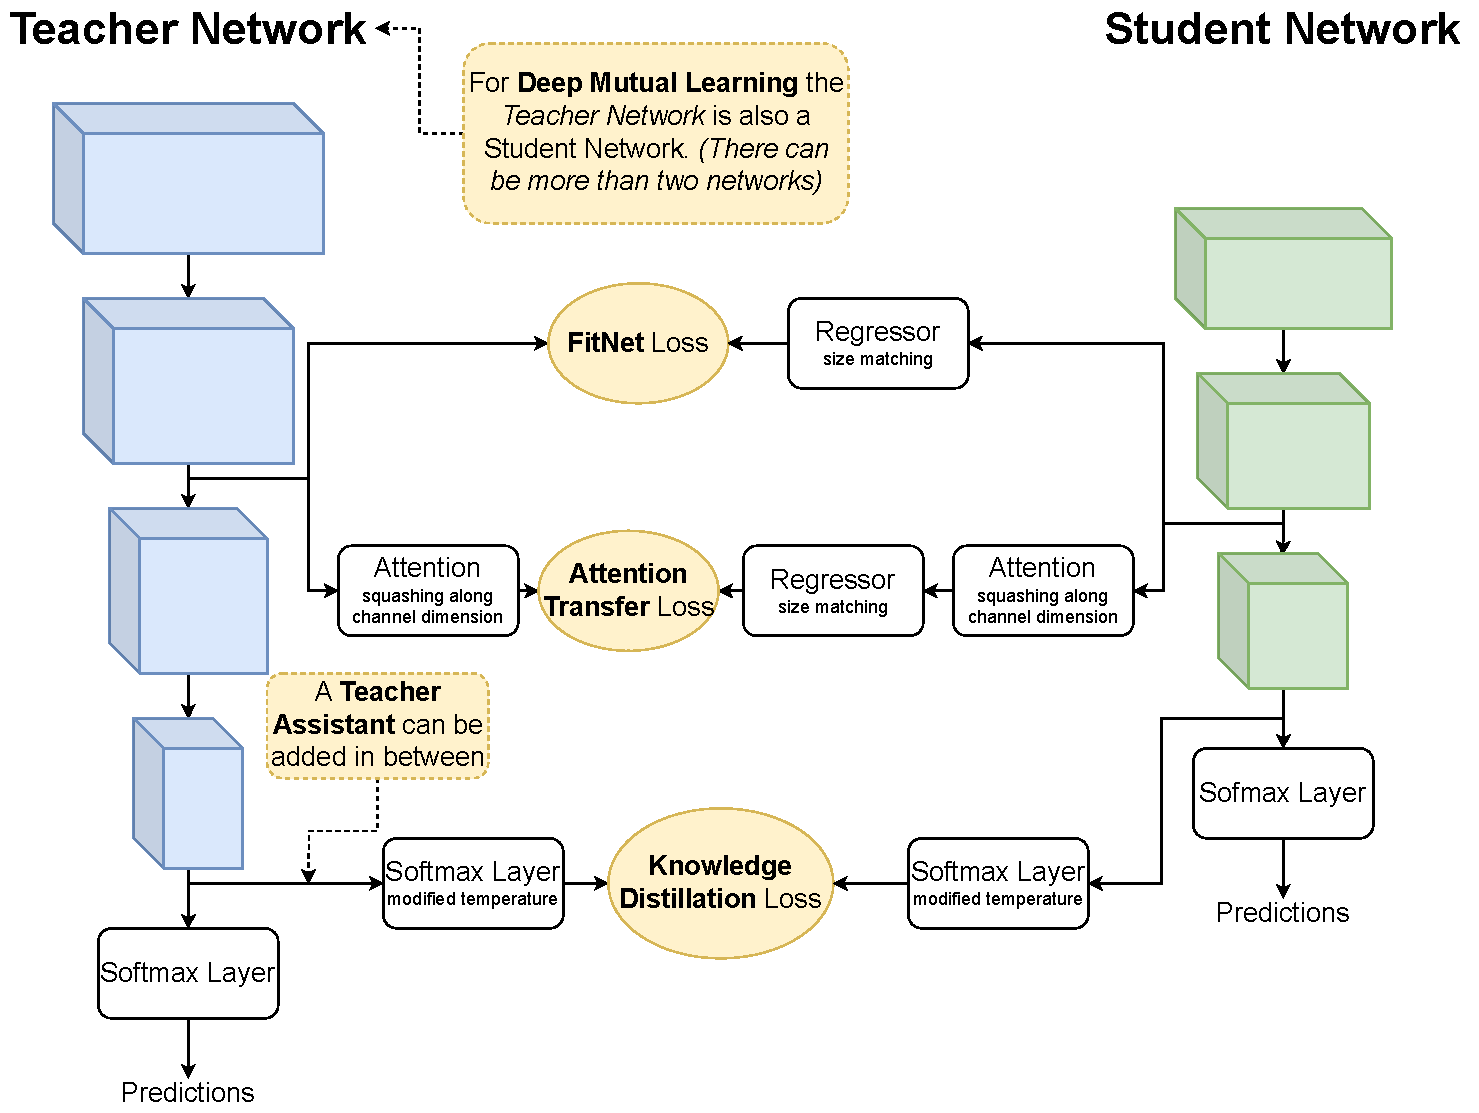
\includegraphics[width=0.75\textwidth]{chapter_sota/assets/kd_frameworks.pdf}
%     \caption{Overview of various knowledge distillation frameworks. From top to
%     bottom, left to right: Deep Mutual Learning
%     \cite{DBLP:conf/cvpr/ZhangXHL18}, FitNet
%     \cite{DBLP:journals/corr/RomeroBKCGB14}, Attention Transfer
%     \cite{DBLP:conf/iclr/ZagoruykoK17}, Teacher Assistant
%     \cite{DBLP:conf/aaai/MirzadehFLLMG20} and Knowledge Distillation
%     \cite{DBLP:journals/corr/HintonVD15}.}
%     \label{fig:sota:kd_frameworks}
% \end{figure}

% In practice, handling full-dimensional feature maps is cumbersome. That is why,
% in order to avoid this issue, \cite{DBLP:conf/iclr/ZagoruykoK17} use an
% attention map generated by squashing the feature maps to a 2D map allowing for a
% smaller 2D regressor to match attention map dimensions. Note that the
% aforementioned knowledge transfer methods require teacher-student pairs and
% assume that teachers are large trained models. \cite{DBLP:conf/cvpr/ZhangXHL18}
% relax this assumption by proposing Deep Mutual Learning, which enables a pool
% of networks of different architectures to learn together, provided that they
% have the same logit dimensions, and none of the models in the pool requires a
% pretraining step. The uncertainty of each model is distilled to each other,
% which creates additional knowledge.\\

% In all the aforementioned methodos, the efficacy of knowledge distillation, and
% consequently, the final performance of the student network, is significantly
% influenced by the disparity in size between the student and teacher networks.
% When this size discrepancy is excessive, the student network may encounter
% difficulties in adequately aligning with the teacher logits, thus preventing
% optimal knowledge distillation. In order to tackle this issue,
% \citeauthor{DBLP:conf/aaai/MirzadehFLLMG20} introduced the concept of
% \emph{Teacher Assistant}: networks of intermediary dimensions that aim at
% bridging the gap between student and teacher
% \cite{DBLP:conf/aaai/MirzadehFLLMG20}. Knowledge is first distilled from the
% teacher to the teacher assistant, and then from the teacher assistant to the
% student, resulting in improved performances compared to straightforward \ac{KD}.\\

% \begin{figure}[htbp]
%     \centering
%     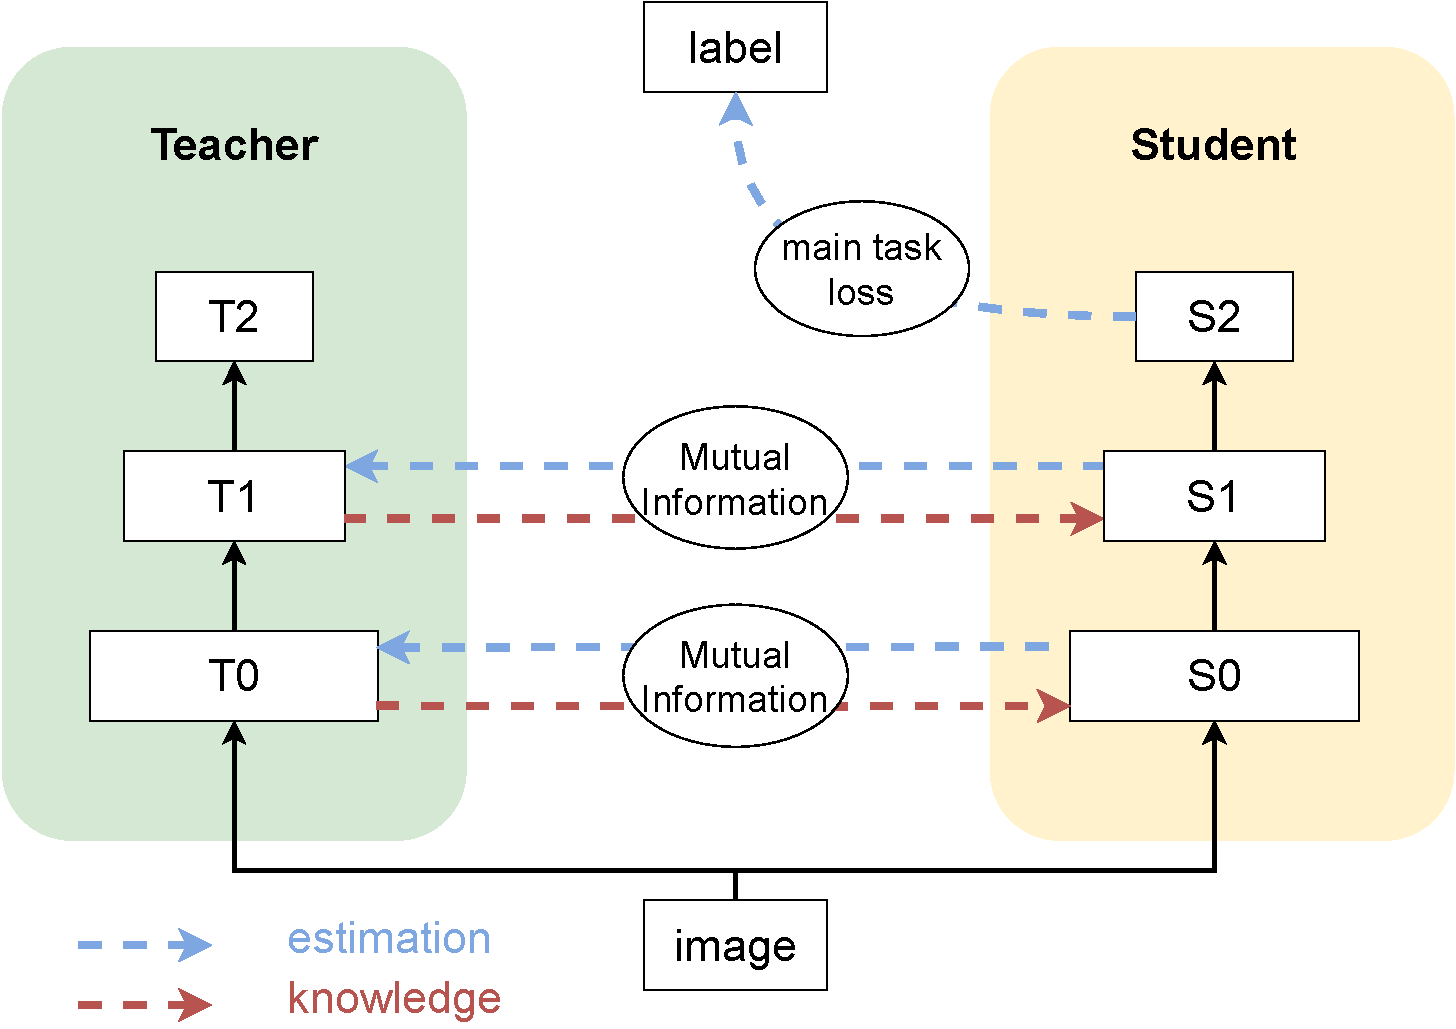
\includegraphics[width=0.7\textwidth]{chapter_sota/assets/variational_info_distillation.pdf}
%     \caption{Conceptual scheme of \cite{DBLP:conf/cvpr/AhnHDLD19}. The student
%     network efficiently learns the main task while retaining high mutual information
%     with the teacher network. The mutual information is maximised by learning to
%     estimate the distribution of the activations in the teacher network, provoking
%     the transfer of knowledge. Adapted from the original
%     scheme found in \cite{DBLP:conf/cvpr/AhnHDLD19}}
%     \label{fig:sota:vid_scheme}
% \end{figure}

% Other approaches that do not rely on direct feature map or logit matching have
% been proposed. \cite{DBLP:conf/cvpr/AhnHDLD19} introduced Variational
% Information Distillation, which indirectly maximises the mutual information
% between the student and the teacher. This is done by using \emph{variational
% information maximisation} \cite{barber2004algorithm} to maximise a variational
% lower bound of the mutual information, since directly maximising the latter is
% intractable in practice (see \cref{fig:sota:vid_scheme}). Likewise,
% \cite{DBLP:conf/eccv/PassalisT18} proposed a Probabilistic Knowledge Transfer
% method that does not match logits or feature maps, but rather represents the
% latter as a probability distribution and minimises divergence between the two
% (see \cref{fig:sota:pkt_scheme}).\\


% \begin{figure}[htbp]
%     \centering
%     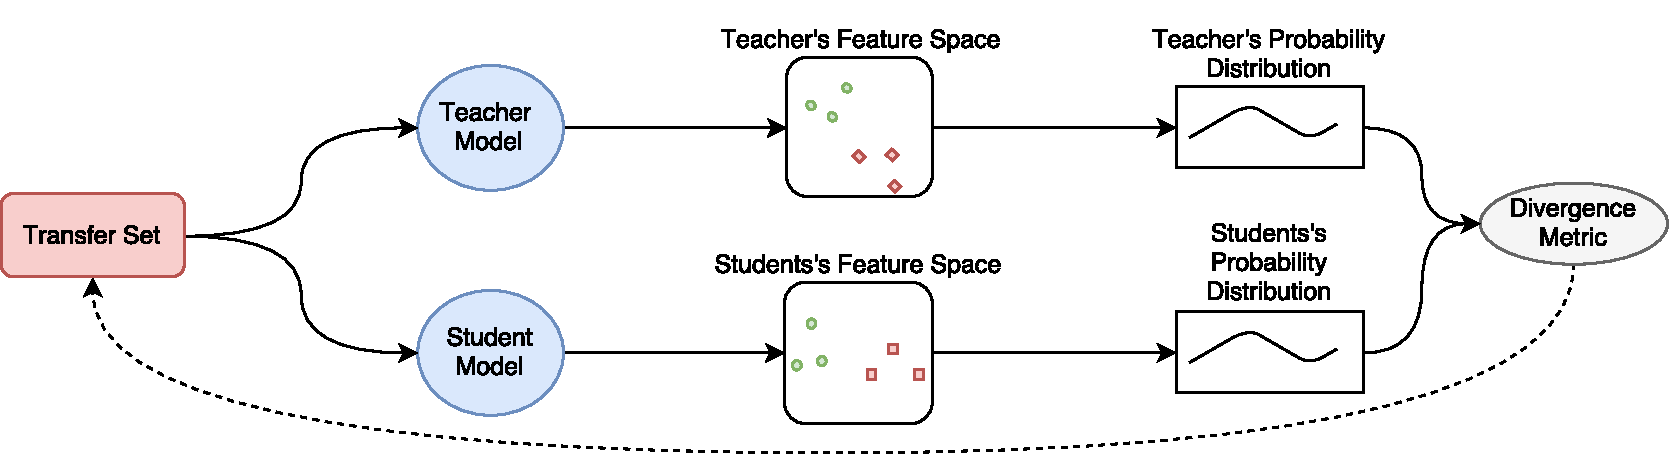
\includegraphics[width=0.7\textwidth]{chapter_sota/assets/pkt_diagram.pdf}
%     \caption{Conceptual scheme of the
%     Probabilistic Knowledge Transfer method. Both the student and the teacher
%     feature maps are modelled using probability distributions. The divergence of the
%     latter is minimised in order to transfer knowledge from the teacher to the
%     student. Illustration taken from \cite{DBLP:conf/eccv/PassalisT18}.}
%     \label{fig:sota:pkt_scheme}
% \end{figure}

% \section*{Alternative Algorithms for Reducing Computational Complexity of Convolutions}
% \label{sec:sota:fast_convolutions}

% Aside from reducing the number of weights, it is also possible to reduce the
% computational complexity of convolutions by using alternative algorithms to
% perform the convolution operation.\\

% The most popular ones rely on the \ac{FFT}
% \cite{DBLP:conf/nips/ChiJM20,DBLP:journals/npl/LinY19,DBLP:conf/pkdd/PrattWCZ17},
% and leverage the Convolution Theorem. The Convolution Theorem states that the
% convolution of two signals in the source domain is the product of the two
% signals in the Fourier domain. This allows for a faster computation of the 2D
% convolution by using the \ac{FFT} to compute the convolution in the frequency
% domain \cite{oppenheim1997signals}.\\


% Other algorithms focus on optimising matrix operations, such as the Strassen
% algorithm \cite{strassen1969gaussian}, used in \cite{DBLP:conf/icann/CongX14}.
% It is a fast method for matrix multiplication that reduces the computational
% complexity from the standard $\mathcal{O}(n^{3})$ to approximately
% $\mathcal{O}(n^{2.807})$ by recursively dividing the matrices of size $n$ into 4
% submatrices of size $\frac{n}{2} \times \frac{n}{2}$, reorganising and combining
% these multiplications to perform only 7 instead of 8 matrix multiplications. The
% Strassen algorithm has later been refined by \citeauthor{coppersmith1987matrix},
% who introduced the Coppersmith-Winograd algorithm \cite{coppersmith1987matrix}.
% The latter brings down the complexity to $\mathcal{O}(n^{2.376})$. This
% algorithm is used in various works, mostly targeted towards a specific \ac{FPGA}
% architecture \cite{liu2018efficient,lu2018spwa,wang2020winonn}.\\


% Another technique for optimising convolutions is the use of Toeplitz matrices. A
% Toeplitz matrix, or diagonal-constant matrix, has the unique characteristic of
% each descending diagonal from left to right being constant. $T$ is an example of
% a Toeplitz matrix. This property is particularly useful for convolutions, as
% they can be expressed as a multiplication by a Toeplitz matrix
% \cite{gray2006toeplitz}. This algorithm has been used in
% \cite{liao2019compressing}, with a focus on \ac{FPGA} architectures. Note that
% the representation of a convolution as a product with a Toeplitz matrix can
% further be accelerated by using the aforementioned optimisations to the matrix
% multiplication algorithm.\\


% $$
% T = 
% \left(
% \begin{array}{cccc}
% a & b & c & d \\
% e & a & b & c \\
% f & e & a & b \\
% g & f & e & a \\
% \end{array}
% \right)
% $$

% All the techniques presented in this section allow speeding up the computation
% of convolution operations, however, they require relatively large matrices to be
% truly efficient. They are not widely used with the current architectures
% \cite{DBLP:conf/cvpr/HeZRS16,huang2017densely,liu2018efficient} since they use
% small $3 \times 3$ kernels which would not benefit directly from these
% algorithms.\\


% The algorithms presented in this section offer significant acceleration in the
% computation of convolution operations. However, their optimal efficiency is
% bound to the use of relatively large matrices. Current architectures
% \cite{DBLP:conf/cvpr/HeZRS16, huang2017densely, liu2018efficient} predominantly
% use small $3 \times 3$ kernels, rendering the direct application of these
% acceleration techniques less beneficial. As a consequence, these techniques have
% not gained widespread adoption in contemporary deep learning architectures.

% \section*{Weight Operations}
